\documentclass[tikz,border=5mm]{standalone}
\usepackage{pgfplots}
\usepackage{pgfplotstable}
\pgfplotsset{compat=1.17}

\begin{document}

    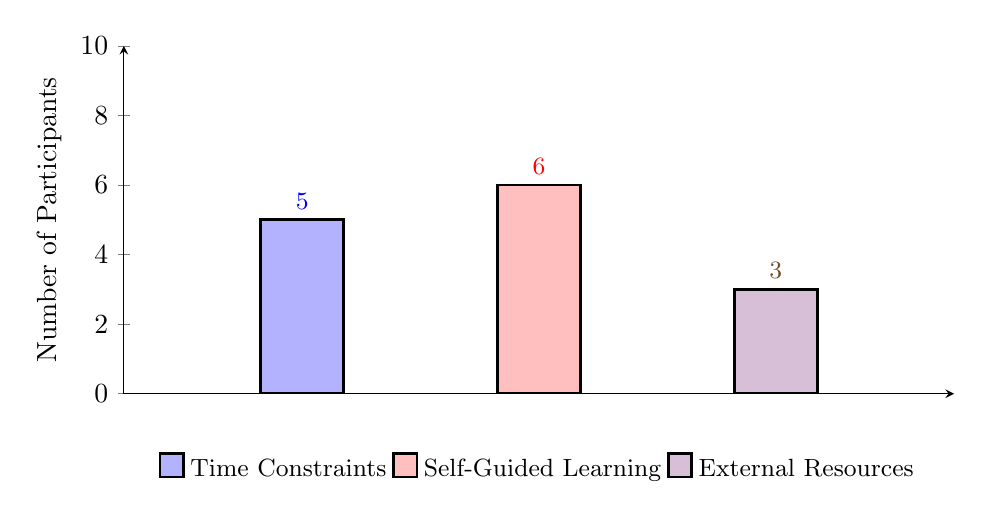
\begin{tikzpicture}
      \begin{axis}[
          ybar,
          symbolic x coords={A,B,C},   % Dummy x coordinates
          xtick=\empty,                 % Remove x-axis tick marks
          axis x line=bottom,           % Draw the x-axis line at the bottom
          axis y line=left,             % Draw the y-axis line only on the left side
          ymin=0, ymax=10,
          bar width=30pt,
          width=\linewidth,             % Ensure the chart fits within a single column
          height=6cm,                   % Adjust height as needed
          enlarge x limits=0.9,         % Add horizontal space between bars
          ylabel={Number of Participants},
          nodes near coords,            % Place numeric labels above each bar
          nodes near coords style={
              font=\color{black}\small, anchor=south
          },
          legend style={
              at={(0.5,-0.15)},
              anchor=north,
              legend columns=3,
              draw=none,
              font=\small,
              nodes={anchor=base}
          },
          legend image code/.code={
              \draw[fill=#1, draw=black] (0cm,0cm) rectangle (0.3cm,0.3cm);
          },
      ]
          % Each \addplot corresponds to one bar, with a black border:
          \addplot+[draw=black, line width=1pt] coordinates {(A,5)};
          \addplot+[fill=pink, draw=black, line width=1pt] coordinates {(B,6)};
          \addplot+[fill=Thistle, draw=black, line width=1pt] coordinates {(C,3)};
          \legend{Time Constraints, Self-Guided Learning, External Resources}
    \end{axis}
    \end{tikzpicture}

\end{document}
